\section{Tensor Core Lines} % (fold)
\label{sec:tcl_theory}
%
The Sujudi/Haimes criterion defines a vortex core line as a structure on which
streamlines have a locally vanishing curvature.
%
The intuition is that in a region where streamlines show a swirling behavior,
there must be a center of rotation where the swirl vanishes.
%
This is fulfilled where the acceleration vector $\mJ\,\vv$ is parallel to the
velocity $\vv$, \ie{}, the flow is accelerated on a straight line.
%
Using this formulation, the criterion can be expressed in terms of the \ac{PV}
operator.
%
To only extract vortex core lines, the Sujudi/Haimes criterion requires an
additional filter criterion.
%
Vortices only occur in regions with swirling flow behavior, which is indicated
by the presence of complex eigenvalues of the Jacobian.
%
Zero-curvature lines also occur in regions where the Jacobian has three real
eigenvalues.
%
These hyperbolic trajectories are the centers of simultaneous converging and
diverging behavior of the vector field and can be used to extract Lagrangian
coherent structures~\cite{Machado2013,Machado2016}
%

%
We apply the idea of Sujudi/Haimes to tensor fields by looking for locations
where the curvature of tensor field lines locally vanishes.
%
We define tensor core lines as the locations where tensor field lines have a
locally vanishing curvature.
%
Note that like vortex core lines, tensor core lines are not generally field
lines of the tensor field.
%
In this section, we provide a formal definition of tensor core lines and
examine their mathematical properties.
%

\subsection{Definition} % (fold)
\label{sub:tcl_definition}
%
Let $\mT(\vx)$ be a \ac{3D} second-order tensor
field that may or may not be symmetric.
%
We want to find locations where the direction of a real eigenvector of $\mT$
does not change when moving along the eigenvector direction, \ie{}, where the
curvature of a tensor field line vanishes.
%
A vector $\vr \neq \vNull$ is a real eigenvector of $\mT$ if $\mT\,\vr = \lambda
\vr$ for eigenvalue $\lambda \in \RRSet$.
%
To observe the change of eigenvector direction when moving along $\vr$,
we need to consider the derivative of $\mT$ in this direction.
%
The directional derivative of $\mT$ along $\vr$, which we write as $\nabla_\vr
\mT$, is the linear combination of three component-wise derivatives
%
\begin{equation*}
    \nabla_{\vr}\mT(\vx) = \nabla \mT(\vx)\,\vr
        = \frac{\partial \mT(\vx)}{\partial x_1} r_1
        + \frac{\partial \mT(\vx)}{\partial x_2} r_2
        + \frac{\partial \mT(\vx)}{\partial x_3} r_3 \,\text{,}
\end{equation*}
%
for $\vx = \T{(x_1, x_2, x_3)}$ and $\vr = \T{(r_1, r_2, r_3)}$.
%

%
Given $\nabla_{\vr}\mT$ we can approximate the behavior of $\mT$ along
$\vr$ as
%
\begin{equation}
\label{eq:lin_approx}
    \mT(\vx + h\vr) = \mT(\vx) + h \nabla_{\vr}\mT(\vx) \,\text{,}
        \quad \text{with} \quad h \in \RRSet \,\text{.}
\end{equation}
%
For our zero-curvature requirement to be fulfilled, the eigenvector direction
must not change when moving along $\vr$, \ie{},
%
\begin{equation}
\label{eq:lin_cond}
    \mT(\vx + h\vr)\,\vr
        = \mT(\vx)\,\vr + h \nabla_{\vr}\mT(\vx)\,\vr
        = \mu \vr\, \text{,} \quad \text{with} \quad \mu \in \RRSet \,\text{.}
\end{equation}
%
This means that $\vr$ is still an eigenvector of $\mT$ (with eigenvalue $\mu$)
at the slightly offset position $\vx + h\vr$.
%
If we substitute $\mT(\vx)\,\vr = \lambda \vr$, we get
%
\begin{align*}
    \lambda \vr + h \nabla_{\vr}\mT(\vx)\,\vr &= \mu\, \vr \\
    \nabla_{\vr}\mT(\vx)\,\vr &= \frac{\mu-\lambda}{h}\, \vr\, \text{,}
\end{align*}
%
\ie{}, $\vr$ is also an eigenvector of $\nabla_{\vr} \mT(\vx)$.
%
With this, a tensor core line is an isolated line of positions $\vx$ where
%
\begin{equation*}
    \lambda \mT(\vx) \, \vr = \mu \nabla_{\vr}\mT(\vx)\,\vr = \vr \text{,}
\end{equation*}
%
for $\vr \neq \vNull$ and $\lambda,\, \mu \in \RRSet$.
%
In terms of the \ac{PV} operator, tensor core lines can then be expressed as
%
\begin{equation}
\label{eq:tensor_line}
    \operatorname{TCL}(\mT) =
        \{\vx\;|\: \exists \;\vr \in \RRSet,\,
        \vr \parallel \mT(\vx)\,\vr \parallel \nabla_{\vr}\mT(\vx)\,\vr
        \land \vr \neq \vNull\} \,\text{.}
\end{equation}
%
In words: a tensor core line is located where an eigenvector $\vr$ of $\mT$ is
parallel to an eigenvector of the directional derivative of $\mT$ along $\vr$.
%
Note the similarity of this criterion to Sujudi/Haimes, which states that a
vortex core lines is located where a vector $\vv$ of the vector field is
parallel to the directional derivative of the field along $\vv$, which is
defined by the acceleration $\mJ(\vv)\,\vv$.
%
In fact, the criterion is almost a straightforward application of the \ac{PEV}
operator we presented in \cref{cha:parallel_eigenvectors}.
%
However, the second tensor field $\nabla_{\vr}\mT$ is dependent on the unknown
$\vr$, which requires a slightly different solution strategy.
%

\begin{figure}
    \begin{captionbeside}
        {Example of seven distinct core lines in a random linear tensor field.
        \label{fig:7lines}}
        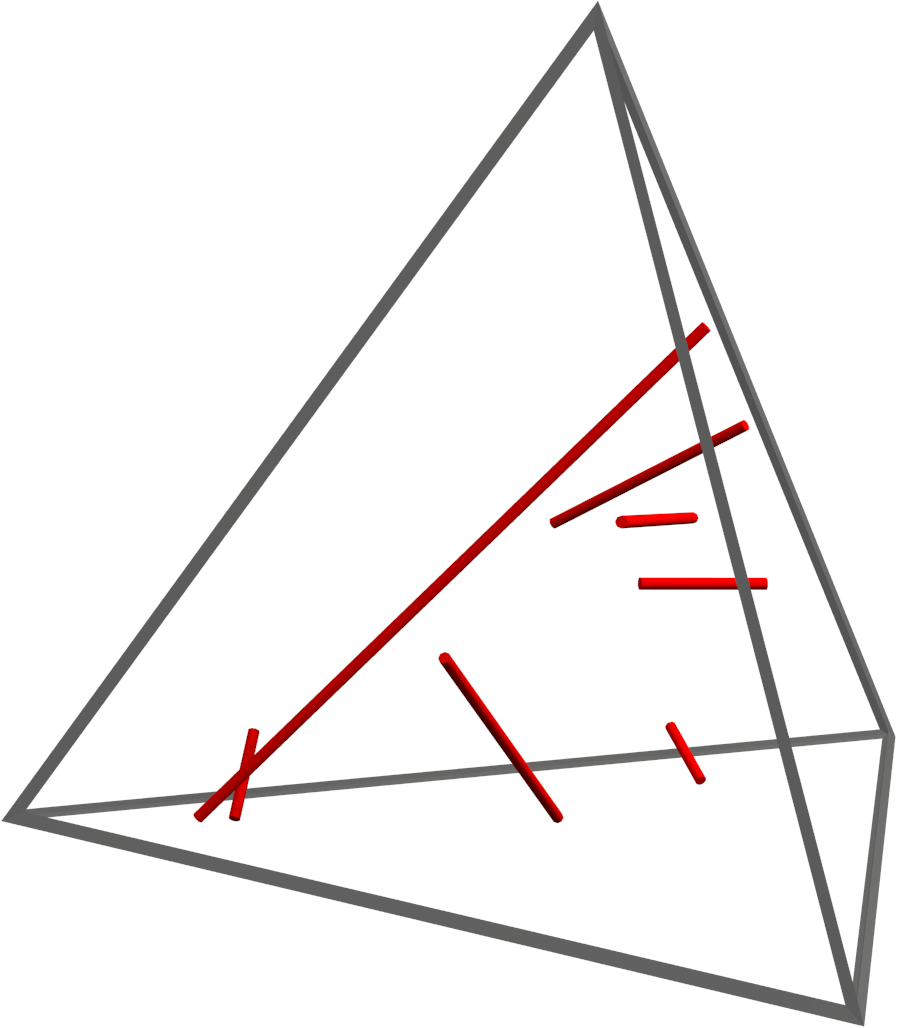
\includegraphics[width=0.5\columnwidth]{figures/7lines}
    \end{captionbeside}
\end{figure}
%
% subsection definition (end)

\subsection{Mathematical Properties} % (fold)
\label{sub:mathematical_properties}
%
We now examine the mathematical properties of tensor core lines.
%
We show that they are indeed structurally stable lines, and that in linear
tensor fields, these lines are always straight.
%

%
\begin{theorem}\label{thm:tcl_stable_lines}
In a $C^1$-continuous tensor field, tensor core lines are structurally stable
line structures that are either closed or end at the domain boundary.
\end{theorem}
%
To show \cref{thm:tcl_stable_lines}, we consider a local representation of a
real eigenvector field in the neighborhood of a point as a normalized vector
field.
%
Then the fact that the \ac{PV} operator gives such line
structures~\cite{Peikert1999} shows the theorem.
%
Note that although such a representation of an eigenvector field as a normalized
vector field is locally possible, it does not apply globally in a consistent
way, and therefore does not provide a strategy to extract tensor core lines.
%
We also mention that in real datasets, tensor cores may build surfaces or even
volumetric structures.
%
This is due to shape symmetries often observed in artificial data produced by
humans.
%
Even though these structures are unstable (adding noise destroys the surfaces to
many lines), our extraction algorithm has to deal with them.
%

%
\begin{theorem}
In linear tensor fields, tensor core lines are straight lines.
\end{theorem}
%
This follows from the fact that for linear tensor fields, the linear
approximation in \eqref{eq:lin_approx} describes the whole data set
exactly: if \eqref{eq:lin_cond} holds for a small $h$, it holds for all
$h$ (i.e., on a whole straight line) as well.
%
\Cref{fig:7lines} shows an example of a random linear tensor field containing
seven isolated tensor core lines.
%
% subsection mathematical_properties (end)